\subsection{Validar y publicar una ley en el portal de edición}

\begin{figure}[H]
\centerline{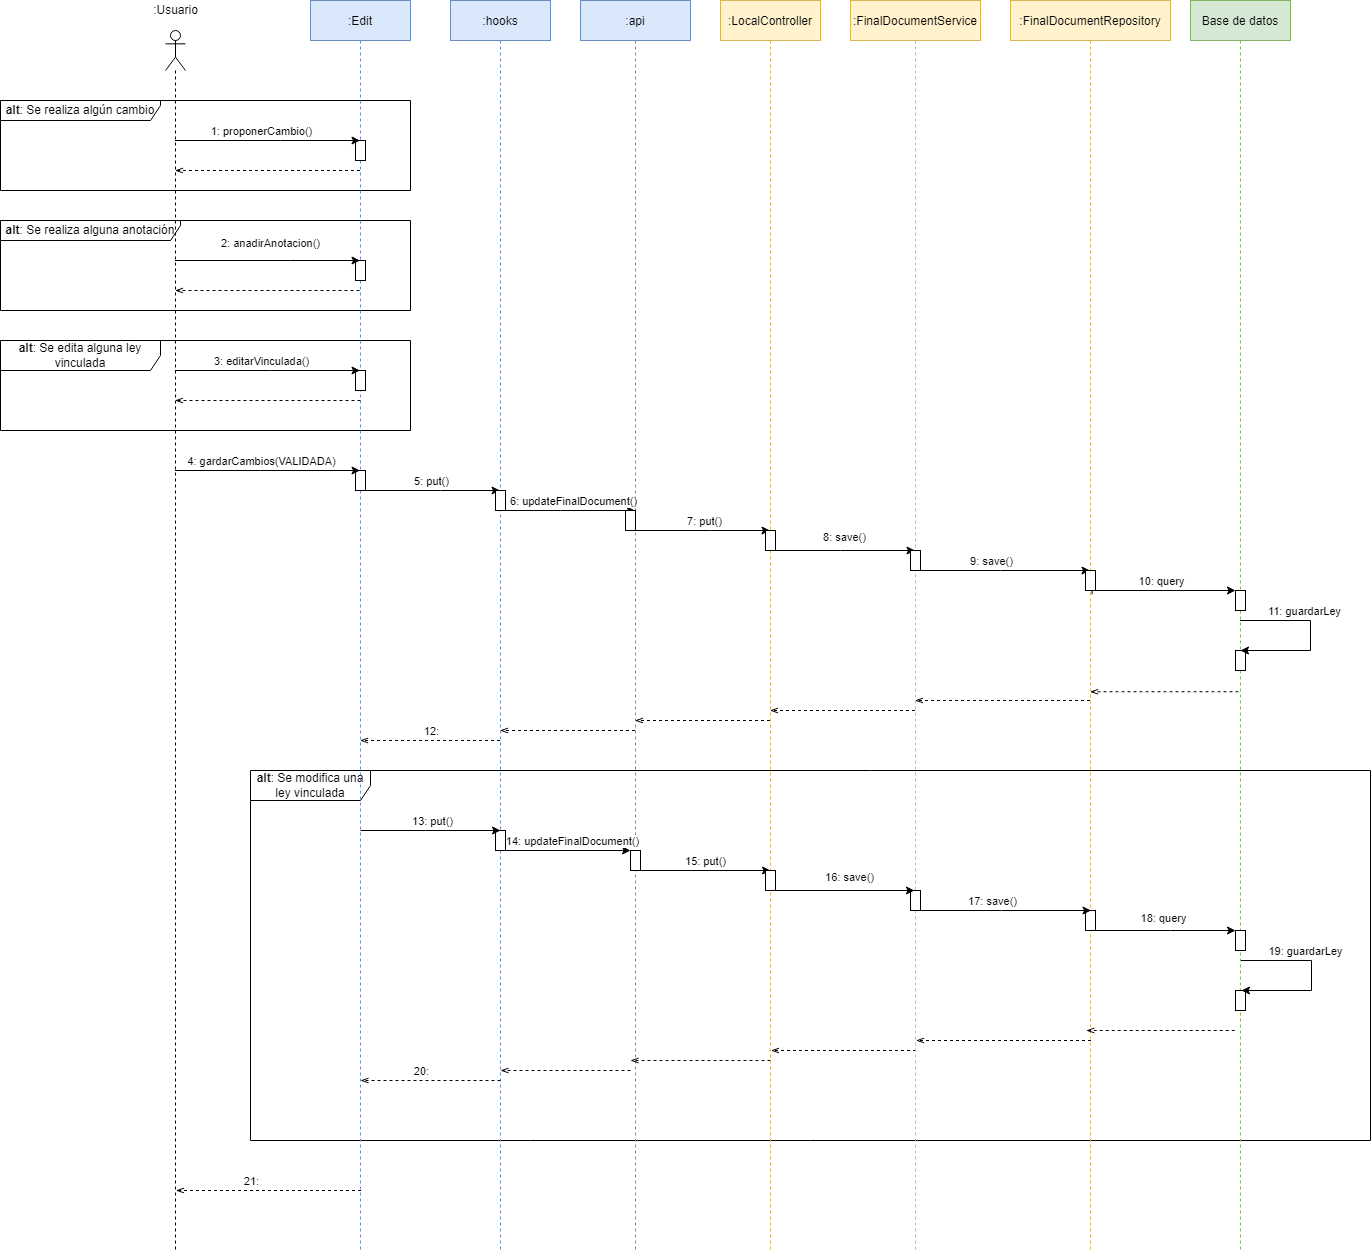
\includegraphics[width=15cm]{figuras/diseño/ValidarLey.png}}
\caption{Diagrama de secuencia de la validación y publicación de una ley en el portal.}
\label{enlaceDValidarLEXGALCuerpo}
\end{figure}

La principal funcionalidad de esta aplicación es la de editar una ley de lex.gal. En esta, un usuario estará visualizando una ley de lex.gal, y procederá a editar sus datos, así como los de las leyes vinculadas. En la \hyperref[enlaceDValidarLEXGALCuerpo]{Figura 3.12} se ilustra el diagrama de secuencia de la operación de validar y publicar una ley de lex.gal, que se puede resumir en los siguientes pasos:

\begin{enumerate}
    \item El usuario puede proponer o no cambios en la página {\bf Edit}.
    \item El usuario puede añadir o no anotaciones en la página {\bf Edit}.
    \item El usuario propone cambios o no en leyes vinculadas en la página {\bf Edit}.
    \item El usuario guarda los cambios. Se utiliza el estado de {\bf VALIDADA} para la ley principal y, en caso de modificar alguna, a sus leyes vinculadas.
    \item Este método invoca al método {\it put()} del hook {\it useFinalDocument()}.
    \item Se invoca al método {\it updateFinalDocument()} de la carpeta  {\bf api}.
    \item Se hace un llamamiento mediante una solicitud HTTP al servidor. En concreto, la función {\it put()} de {\bf LocalController}, pues se hace un PUT. Se comprueba en los filtros que el usuario está autenticado.
    \item Se invoca al servicio {\it save()} de {\bf FinalDocumentService}.
    \item Se invoca la operación {\it save()} del repositorio {\bf FinalDocumentRepository}, para poder modificar una ley.
    \item Se invoca la operación de modificación en la base de datos de MongoDB.
    \item Se modifica la ley correspondiente en la base de datos.
    \item Se procede a devolver la respuesta al cliente desde este paso, realizando el proceso inverso.
    \item En caso de que todo fue correctamente en los pasos anteriores, y que la ley principal modifica alguna ley vinculada, se procede a editar esta correspondientemente. Se repiten todos los pasos descritos desde el punto 5 al punto 12 para la ley vinculada.
    \item Por último, se indica al usuario que se validó y publicó la ley principal, así como las leyes vinculadas si corresponde.
\end{enumerate}